
\documentclass[a4paper,12pt,oneside,pdflatex,italian,final,twocolumn]{article}

\usepackage[utf8]{inputenc}
\usepackage{parallel}
\usepackage{siunitx}
\usepackage{booktabs}
\usepackage{fancyhdr}
\usepackage{caption}
\usepackage{multirow}
\usepackage{gensymb}
\usepackage[export]{adjustbox}
\usepackage[margin=0.5in]{geometry}
\addtolength{\topmargin}{0in}

\usepackage{libertine}
\renewcommand*\familydefault{\sfdefault}  %% Only if the base font of the document is to be sans serif
\usepackage[T1]{fontenc}

\graphicspath{{./images/}}

\title{Piano Datasheet}
\author{Team : Dream Epic }
\date{\today}

\begin{document}

\pagestyle{fancy}

\lhead{ENTC}
\chead {\today}
\rhead{Datasheet v1}

\onecolumn

\begin{figure}
    \begin{minipage}{0.47\textwidth}
        \centering
        
\includegraphics[width=.7\textwidth,left,]{entc_uom_logo.jpg}
    \end{minipage}
    \hfill
    \begin{minipage}{0.47\textwidth}
        \raggedleft
        \Huge \textbf{The Analog Piano}
    \end{minipage}
\end{figure}

\begin{figure}
    \begin{minipage}{0.65\textwidth}
    \section{Overview}
 The device is a sound synthesizer that mimics the sound of c-wave similar to that of a piano, on keypress.  A speaker(8$\Omega$ preferred) ranges around 3W can be used with the pinout to observe the sound output. The volume of the speaker and the noise level can be adjusted according to user interest. The components in the device can be adjusted according to one's interest to mimic a complete piano by implementing many such modules. The amplifier alone can be used to drive small speakers from the low power signal output of simple devices such as mobile phones. 
    \end{minipage}
    \hfill
    \begin{minipage}{0.3\textwidth}
        \centering
        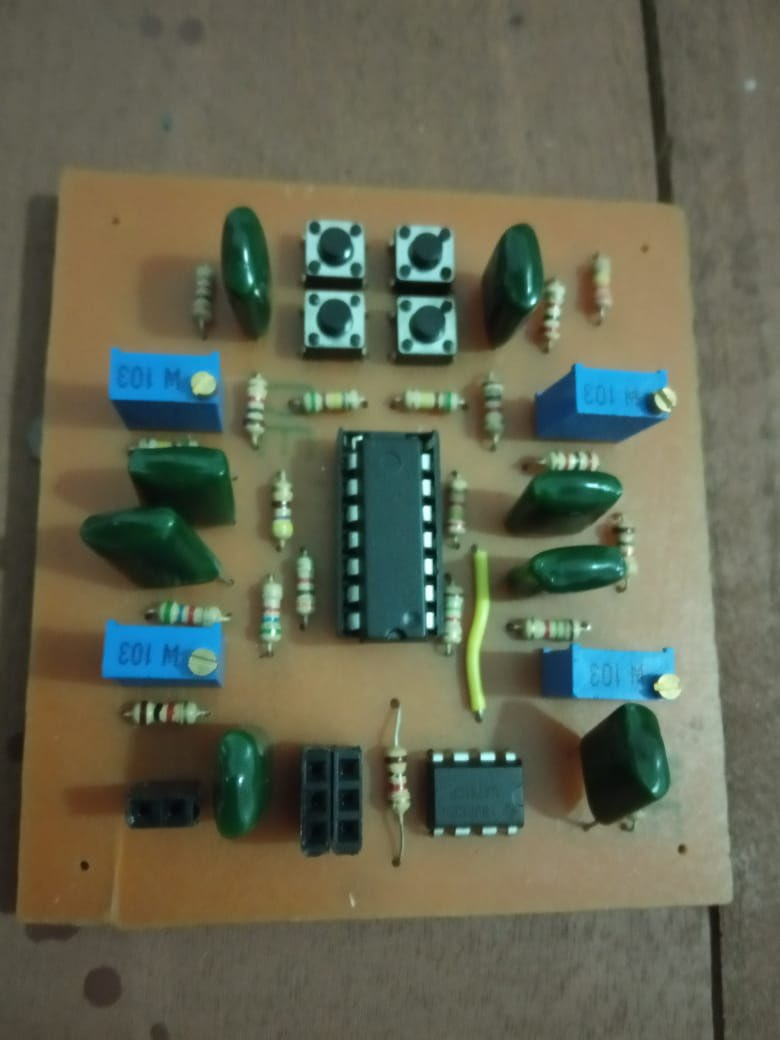
\includegraphics[width=0.85\textwidth,right]{product.jpg}
    \end{minipage}
\end{figure}

\section{Description}
As illustrated in the block diagram below the device consist of four oscillators which are fired by a push button. These oscillators mimic the first four harmonics which are strong enough to model the c-keynote. The triggered signals get added and scaled accordingly through a scalar adder. The output is filtered and amplified before reaching the speaker. Damping time of the wave can be controlled via the damping mechanism attached through a variable resistor with each oscillator. These can be used to mimic the functionality of the damping pedal by increasing their values.
\par
The preset in the amplifier block is allowed to tune by the user to get a noise-free output. For longer usage, it is recommended to keep the preset at a lower value which affects the power efficiency of the circuit. It is expected to use the device not more than fifteen minutes continuously which may harm the operation of the amplifier. Heat sinks used in the amplifier can reach up to 100$\degree$C. It is not advisable to touch them during the continuous operation of the synthesizer.
\par
The maximum current drawn by the oscillator and scalar adder is less than 5mA. Due to such a lower requirement, it is omitted in the technical specifications.
\begin{figure}[h]
    \centering
    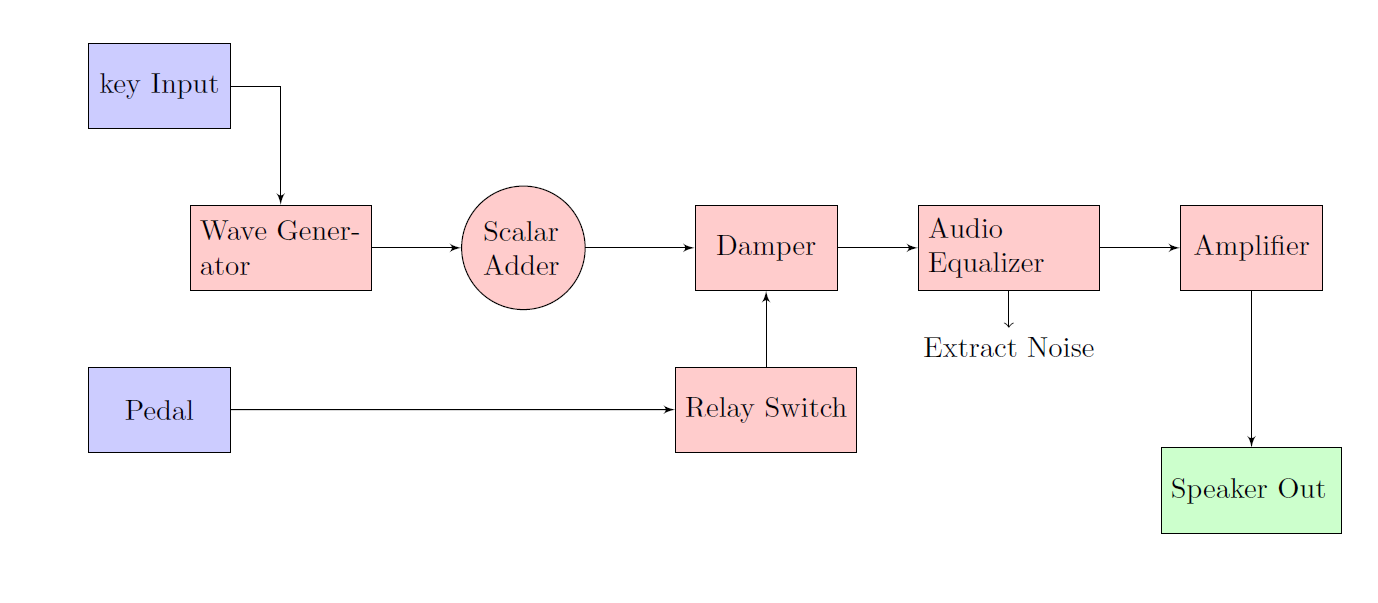
\includegraphics[width=\textwidth]{flow}
    \caption{Circuit Block Diagram}
\end{figure}
\newpage
\section{Technical specification}
Specifications are indicated for each module even though it pin-out of the device is narrower. This is done in the belief of allowing the users to make use of this to combine such modules in the creation of complete piano.\\
\vspace{-.5cm}
\begin{figure}[h]
\begin{minipage}{\textwidth}
\begin{center}
\begin{tabular}{|c|c|c|c|}
     \multicolumn{4}{l}{\textbf{Oscillators}}\\
    \toprule
     Operational  & Operational  & Decaying Control  & Output \\
     Voltage(V) & Frequencies(Hz)& Range(ms) & Impedance($k\Omega$)\\
    \midrule
   \multirow{4}{*}{3-6} & 281$\pm$3 & 300$\pm$100 & 2.49 \\
     & 537$\pm$3 & 300$\pm$120 & 0.44 \\
     & 790$\pm$5 & 300$\pm$150 & 2.37 \\
     & 1100$\pm$5 & 300$\pm$200 & 7.43 \\
    \bottomrule
\end{tabular}
\end{center}
\end{minipage}

\begin{minipage}{\textwidth}
\vspace{.8cm}
\begin{center}
    \begin{tabular}{|c|c|c|c|}
     \multicolumn{4}{l}{\textbf{Scalar Adder}}\\
    \toprule
     Operational  & Allowed Frequency & Recommended Resistance  & Output \\
     Voltage(V) & Range(Hz) & Range($k\Omega$) & Impedance($k\Omega$)\\
    \midrule
    9-12 & 20-20000 & 0.5-50 & 4.53\\
    \bottomrule
\end{tabular}
\end{center}
\end{minipage}

\begin{minipage}{\textwidth}
\vspace{.8cm}
\begin{center}
    \begin{tabular}{|l|c|c|}
     \multicolumn{3}{l}{\textbf{Amplifier}}\\
    \toprule
       & Unit & Value \\
    \midrule
    Operational Voltage & V & 9-12\\
    Current Requirements & A &0.08-0.5\\
    Input Impedance(Ac) & $M\Omega$ & 43$\pm$5\\
    Output Impedance(Ac) & $\Omega$&$10\pm5$\\
    Operational Frequency Range & Hz &200-12000\\
    Volume Control Range & dB & 20-70\\
    Achievable Power Efficiency &  & 63\%\\
    
    \bottomrule
\end{tabular}
\end{center}
\end{minipage}
\end{figure}


\raggedright
\vspace{-.5cm}
\section{Pinout}
\begin{minipage}{.48\textwidth}
\begin{center}
    \begin{tabular}{|c|c|}
     \multicolumn{2}{l}{\textbf{PCB-I : Wave Generator}}\\
    \toprule
        Pin & Signal \\
    \midrule
        \multicolumn{2}{|l|}{P1}\\
    \midrule
    1 & Ground \\
    2 & Power Supply +10.5$\pm$1.5\\
    3 & Power Supply -4$\pm$1\\
    4 & Ground \\
    5 & Power Supply +4$\pm$1\\
    6 & Power Supply -10.5$\pm$1.5\\
    \midrule
        \multicolumn{2}{|l|}{P2}\\
    \midrule
    1 & Signal Out\\
    2 & Ground\\
    \bottomrule
\end{tabular}
\end{center}
\end{minipage}
\begin{minipage}{.48\textwidth}
\begin{center}
    \begin{tabular}{|c|c|}
     \multicolumn{2}{l}{\textbf{PCB-II : Amplifier}}\\
    \toprule
        Pin & Signal \\ 
    \midrule
    \multicolumn{2}{|l|}{P1}\\
    \midrule
    1 & Signal In\\
    2 & Ground\\
    \midrule
    \multicolumn{2}{|l|}{P2}\\
    \midrule
    1 & Power Supply +10.5$\pm$1.5\\
    2 & Audio Out\\
    3 & Ground\\
    4 & Audio Out\\
    5 & Power Supply -10.5$\pm$1.5\\
    \bottomrule
\end{tabular}
\end{center}
\end{minipage}
\newpage
\section{Fine-Tuning}
\vspace{-0.2cm}
\begin{enumerate}
    \item \textbf{Wave Generator} : The resistance values of multi-turn presets  R5, R13, R22, and R2 can be adjusted to achieve different damping time constant of the output wave. These are corresponding to frequencies 1100Hz, 790Hz, 537Hz, and 281Hz respectively. Users also have the flexibility to change R8, R17, R23, and R15 in an inversely proportional manner to vary the proportional constants of those frequencies on the final wave output.
    \vspace{-.3cm}
    \item \textbf{Amplifier} : The resistance value of the preset RP can be adjusted according to the power required to achieve different audio levels in the speaker output. Keeping the resistance values around 2K$\Omega$ is recommended for longer usage.
\end{enumerate}

\vspace{-1cm}
\section{Measurements}
\vspace{-.4cm}
\begin{figure}[h]
    \begin{minipage}{0.45\textwidth}
        \centering
        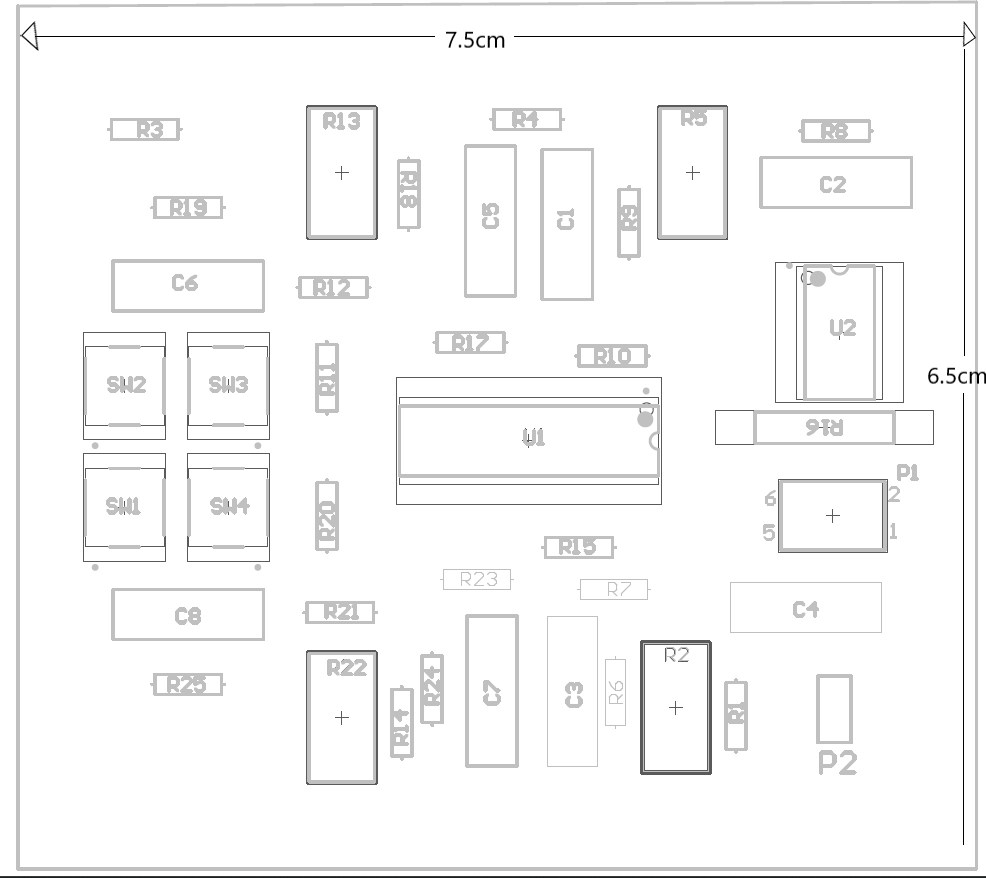
\includegraphics[width=.65\textwidth]{osc_ms}
        \caption*{PCB-I : Wave Generator}
        \label{pcb_1}
    \end{minipage}
        \hfill
        \begin{minipage}{0.45\textwidth}
        \centering
        \includegraphics[width=.65\textwidth]{amp_ms}
        \caption*{PCB-II : Amplifier}
        \label{pcb_2}
    \end{minipage}
\end{figure}
\vspace{-1.3cm}
\section{Application Curves}
\vspace{-.2cm}
The output wave pattern(\ref{wave}) and its spectrum(\ref{spectrum}) at the end of wave generator are indicated in the following figures. The damping time constant can be elongated via the variable resistor attached to each oscillator.
\begin{figure}[h]
    \begin{minipage}{0.47\textwidth}
        \centering
        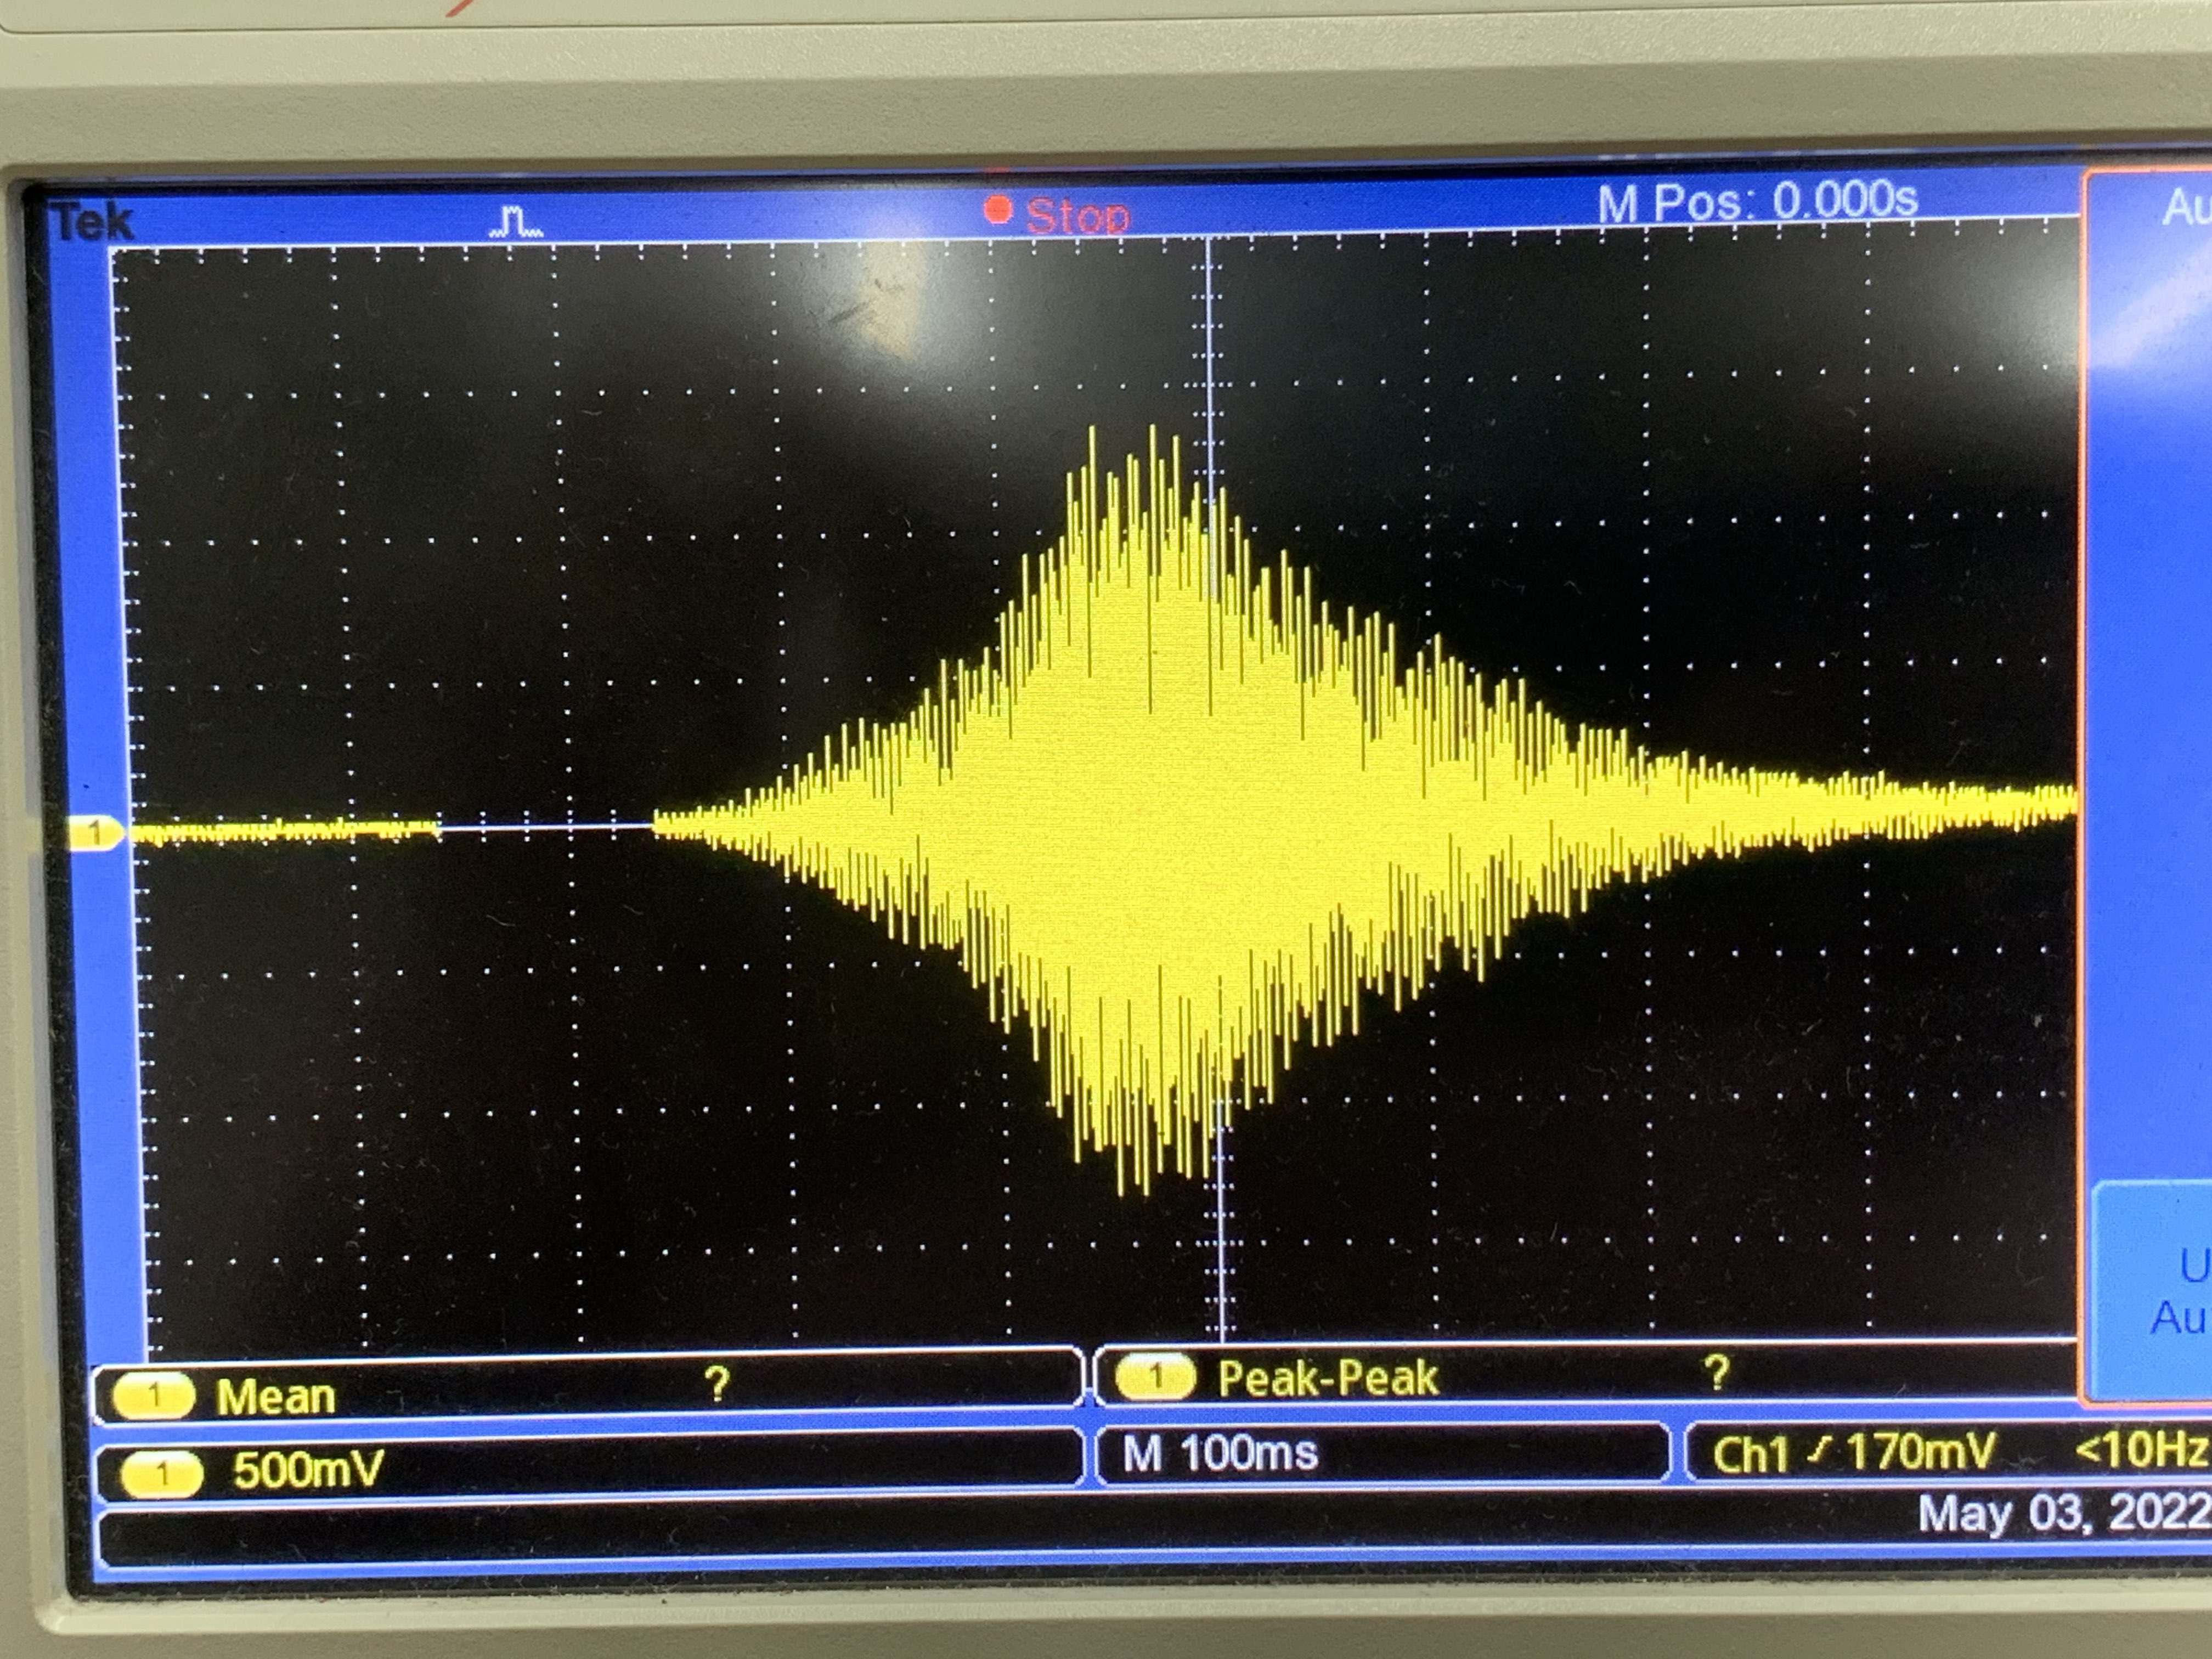
\includegraphics[width=.65\textwidth]{final_wave}
        \caption{Final Wave Pattern}
        \label{wave}
    \end{minipage}
        \hfill
        \begin{minipage}{0.47\textwidth}
        \centering
        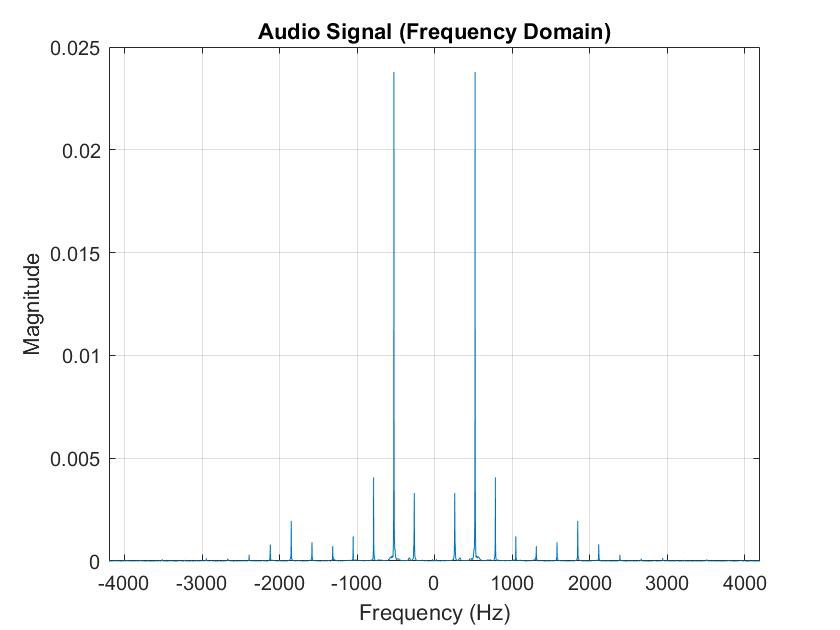
\includegraphics[width=.65\textwidth]{spectrum_c}
        \caption{Frequency Spectrum}
        \label{spectrum}
    \end{minipage}
\end{figure}

The magnitude response(\ref{magnitude}) and phase response(\ref{phase}) of the amplifier are indicated below. The amplifier is suitable for frequencies ranging from 0Hz to 12kHz. This is visible from the facts that the overall gain is maintained at a constant value according to the volume control and the phase is maintained at -180$\degree$ in that range.
\begin{figure}[h]
    \begin{minipage}{0.47\textwidth}
        \centering
        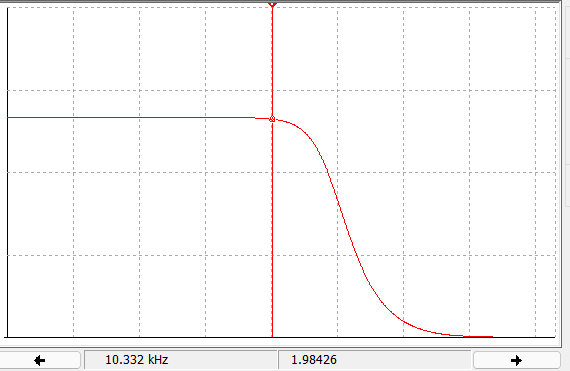
\includegraphics[width=.55\textwidth]{magnitude}
        \caption{Magnitude}
        \label{magnitude}
    \end{minipage}
    \hfill
    \begin{minipage}{0.47\textwidth}
        \centering
        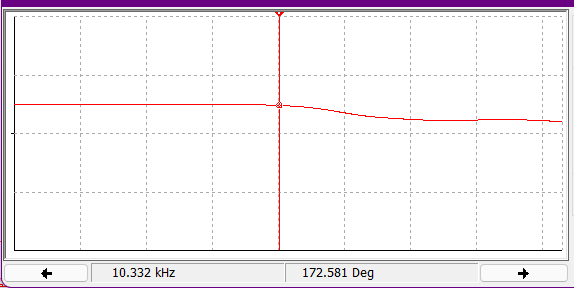
\includegraphics[width=.65\textwidth]{phase}
        \caption{Phase}
        \label{phase}
    \end{minipage}
\end{figure}

\begin{figure}[p]
\begin{center}
\vspace{-4cm}
    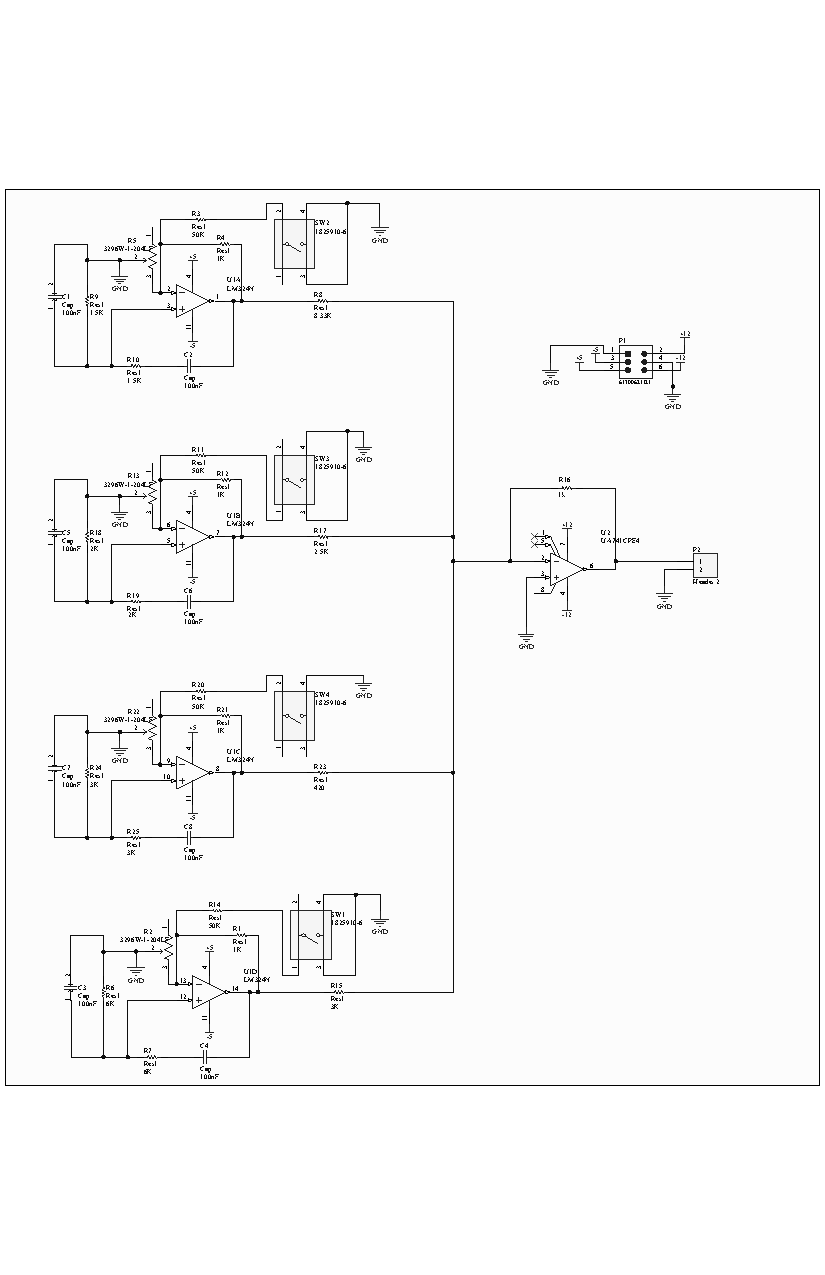
\includegraphics[width=.8\textwidth]{oscillator}
\end{center}
\end{figure}
\begin{figure}[p]
\begin{center}
\vspace{-5cm}
    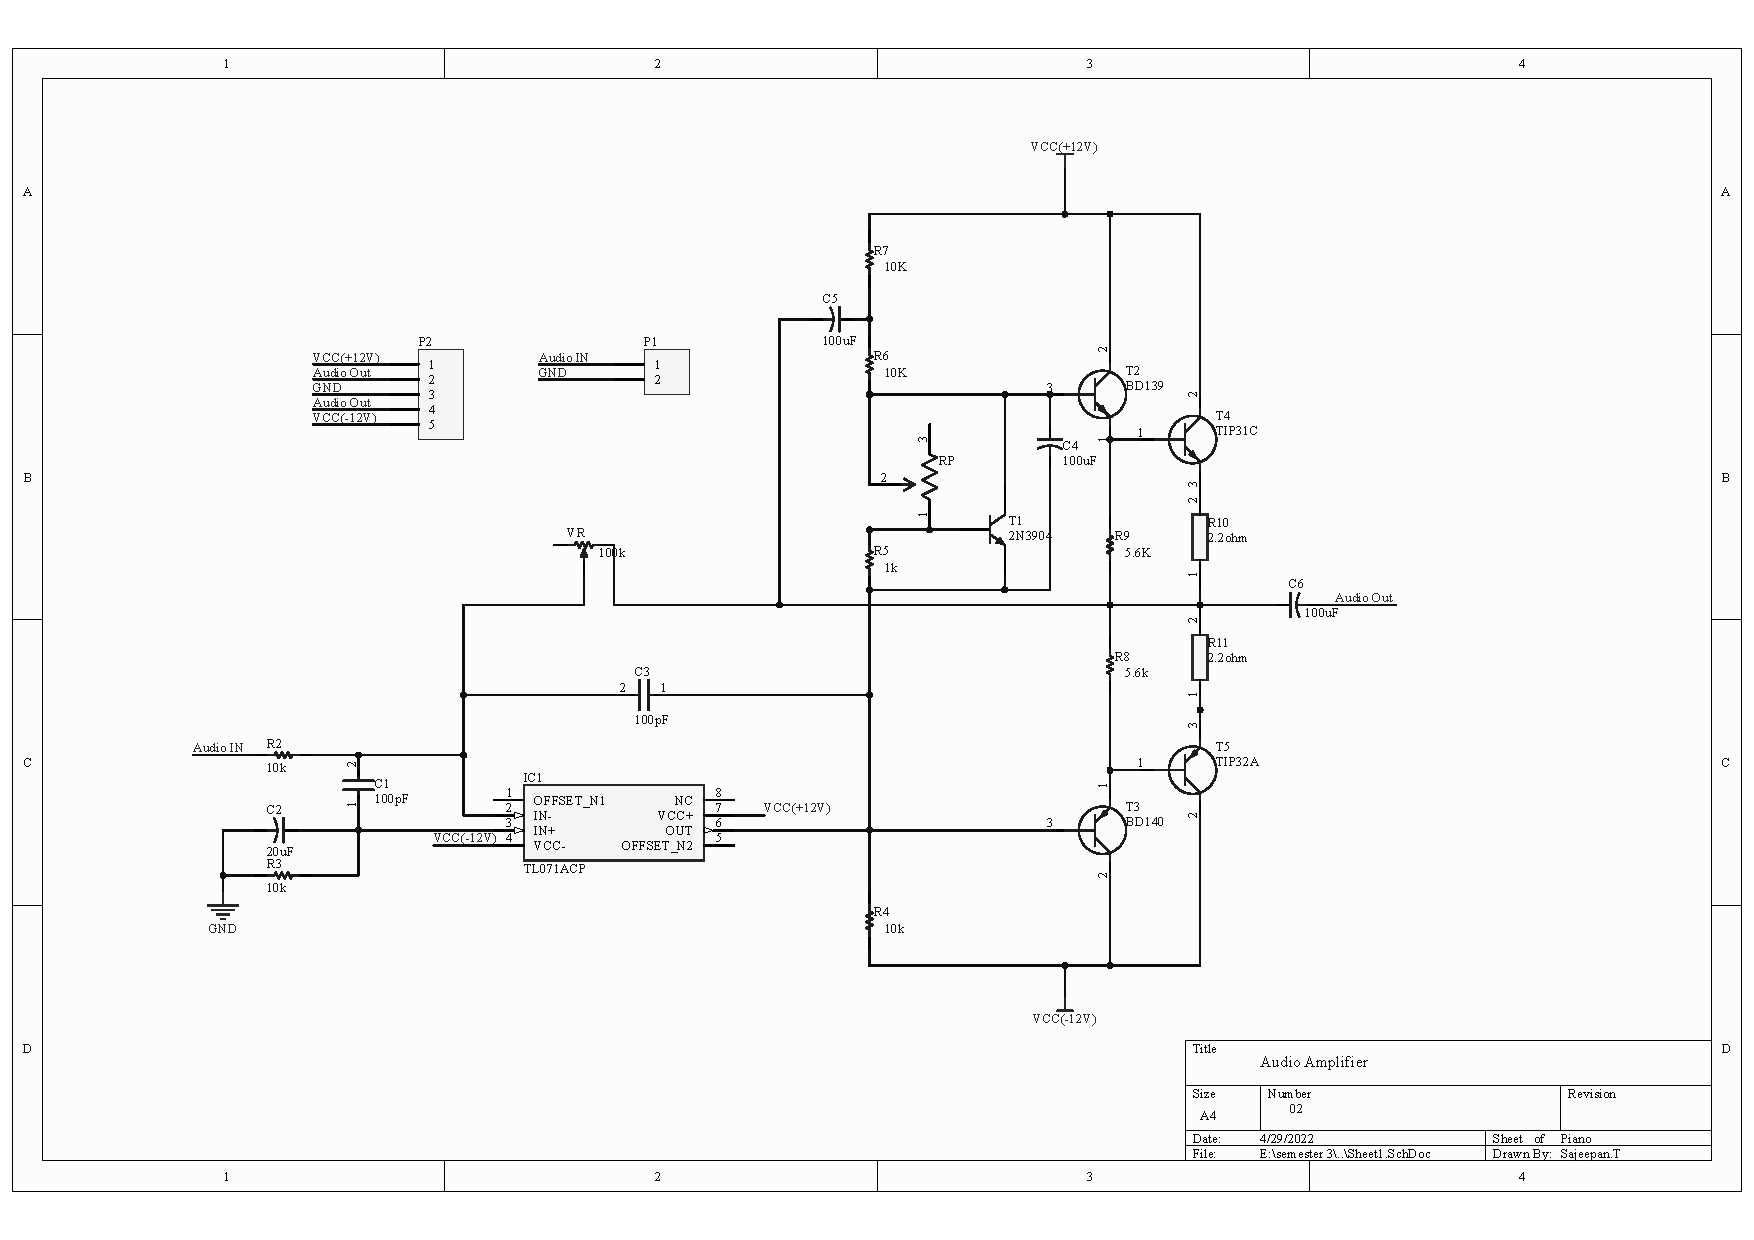
\includegraphics[width=.8\textwidth]{images/amplifier_sch.pdf}
\end{center}
\end{figure}
\end{document}



